% -*-latex-*-

\chapter{Results and Conclusions}
\label{C8}

In this chapter, preliminary results for the proton asymmetries and polarized cross-section differences are presented. The spin structure functions and their contributions to the spin polarizabilities are discussed as well. Only the L-HRS data with 1.710, 2.253 and 3.350 GeV beam energies are analyzed in this thesis. Future work towards final results are described in the end.

\section{Asymmetry Results}
\label{C8S1}

\Cref{C7S1E3,C7S1E4} can be used to extract the physics asymmetry. The beam current has been discussed in \Cref{C5S2SS2} and the livetime correction has been discussed in \Cref{C5S4SS2}. The beam polarization and target polarization has been discussed in \Cref{C5S2SS4} and \Cref{C5S3SS3}, respectively. The preliminary dilution factors have been given in \Cref{C7S4}. Thus, the physics asymmetries can be extracted. The results are shown in \Cref{C8S1F1,C8S1F2,C8S1F3,C8S1F4}.

\begin{figure}[p!]
  \centering
  \begin{subfigure}[t]{0.79\textwidth}
    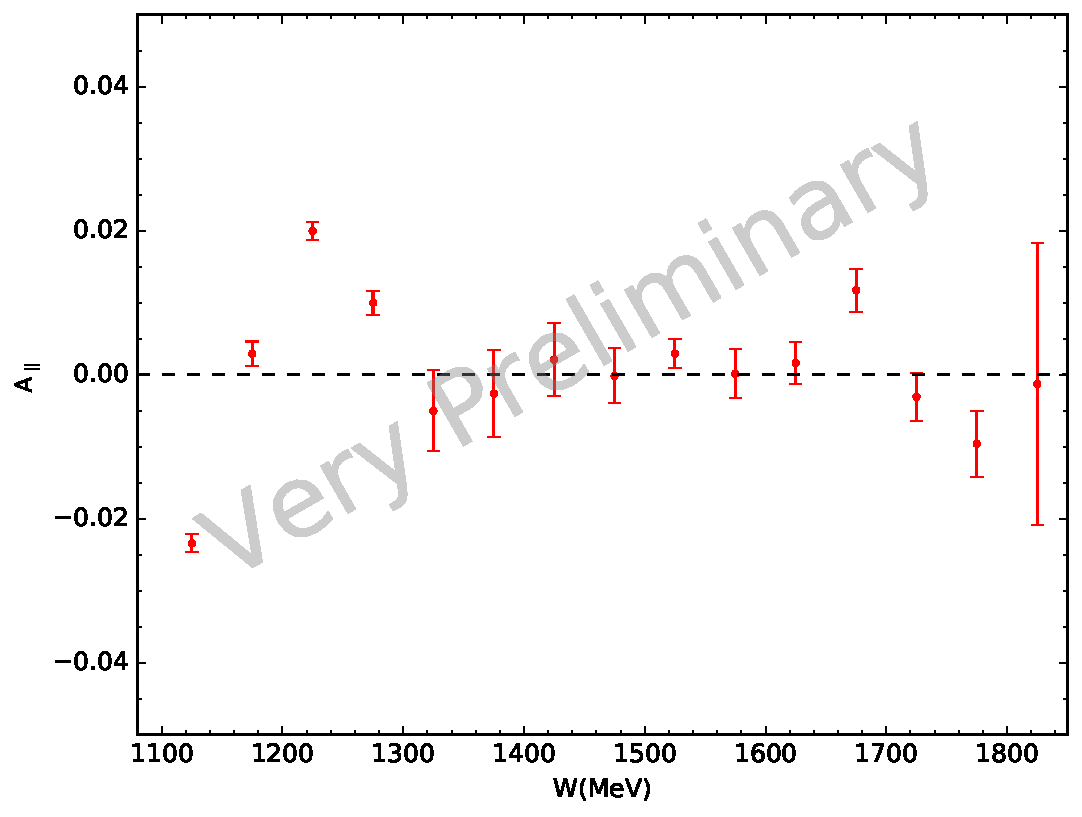
\includegraphics[width=\textwidth]{figs/asymmetry-22535000.pdf}
    \caption{Longitudinal configuration. \label{C8S1F1a}}
  \end{subfigure}
  \begin{subfigure}[t]{0.79\textwidth}
    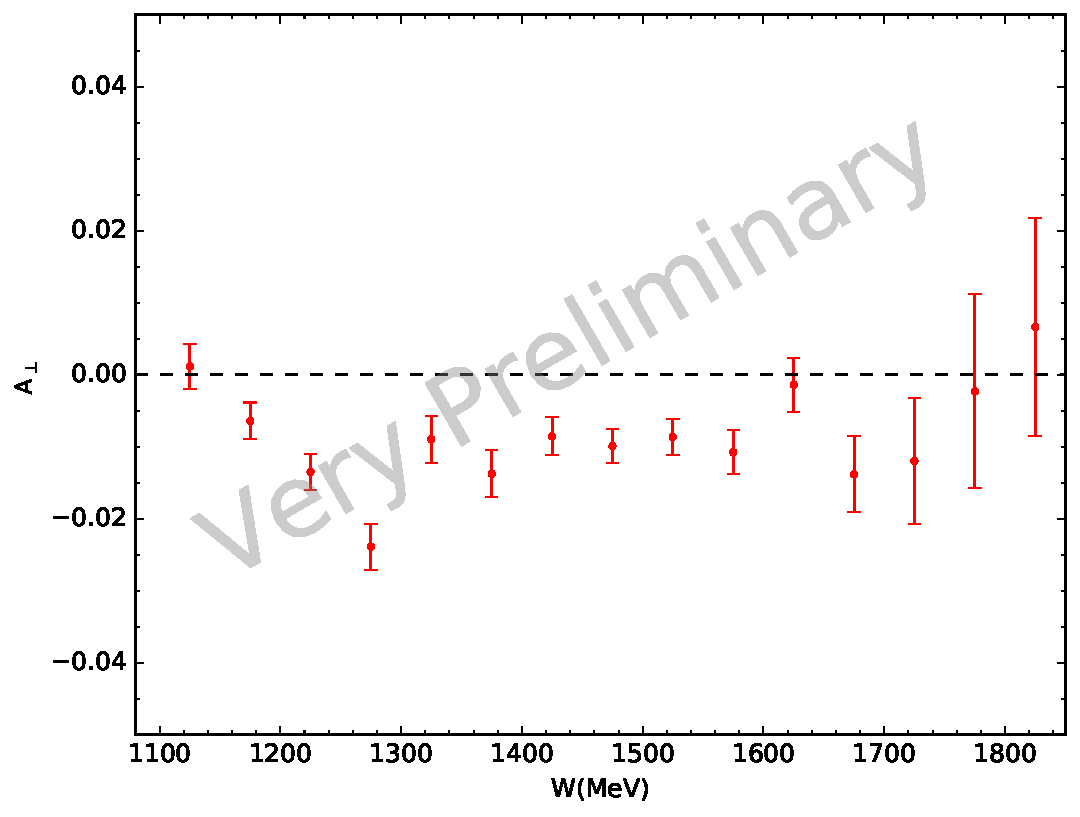
\includegraphics[width=\textwidth]{figs/asymmetry-22535090.pdf}
    \caption{Transverse configuration. \label{C8S1F1b}}
  \end{subfigure}
  \caption[Physics asymmetries with $E=2.253$ GeV and $B=5.0$ T.]{Physics asymmetries for the configurations with 2.253 GeV beam energy and 5.0 T target field. The uncertainties shown are only statistical. \label{C8S1F1}}
\end{figure}

\begin{figure}[p!]
  \centering
  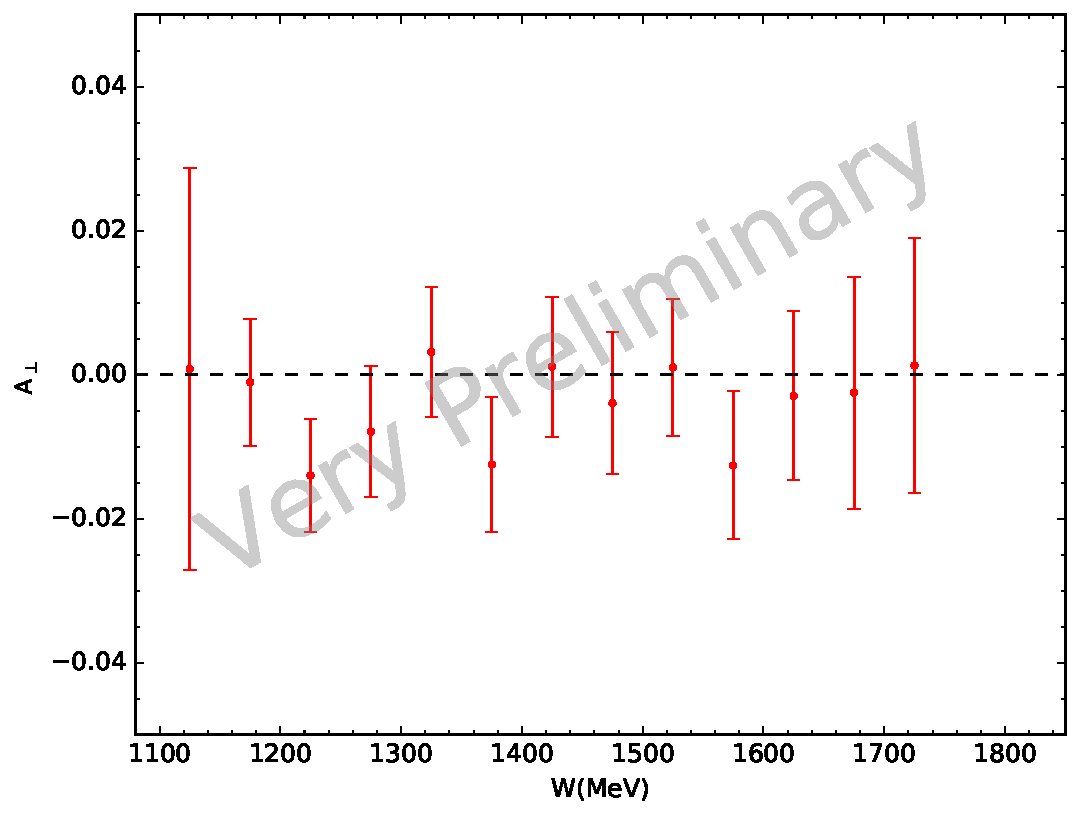
\includegraphics[width=0.79\textwidth]{figs/asymmetry-17102590.pdf}
  \caption[Physics asymmetries with $E=1.710$ GeV and $B=2.5$ T.]{Physics asymmetries for the configurations with 1.710 GeV beam energy and 2.5 T transverse target field. The uncertainties shown are only statistical. \label{C8S1F2}}
\end{figure}

\begin{figure}[p!]
  \centering
  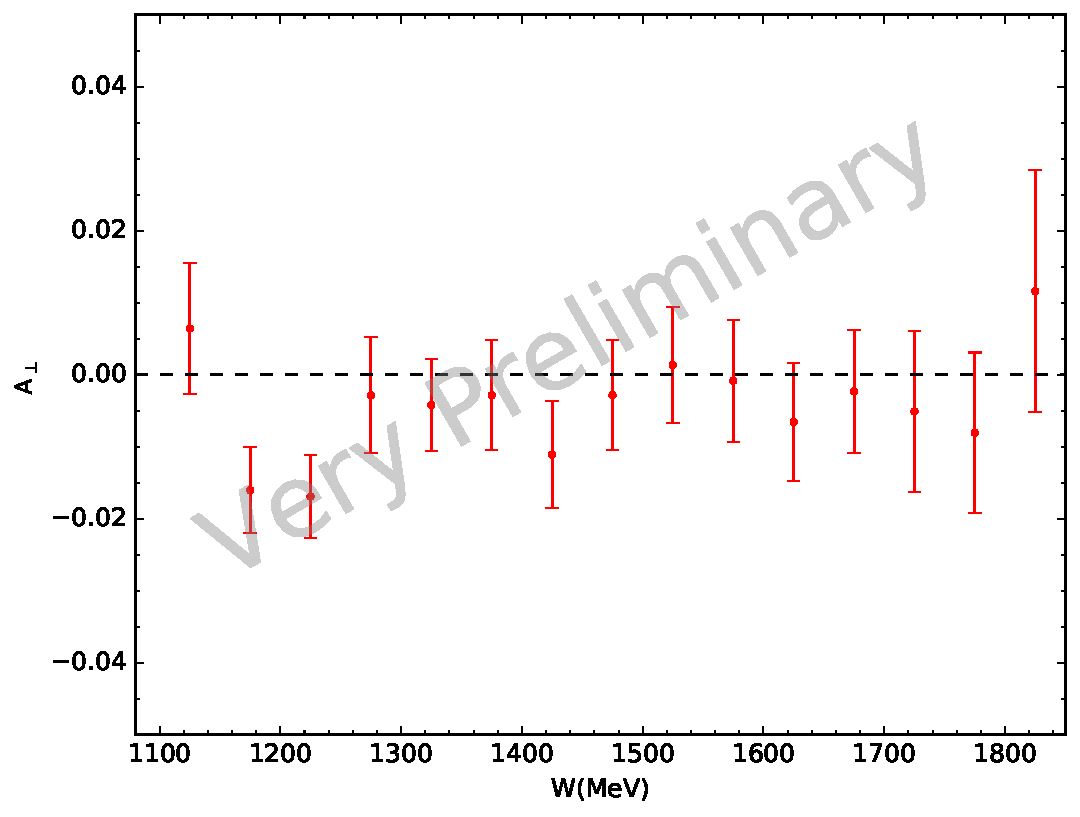
\includegraphics[width=0.79\textwidth]{figs/asymmetry-22532590.pdf}
  \caption[Physics asymmetries with $E=2.253$ GeV and $B=2.5$ T.]{Physics asymmetries for the configurations with 2.253 GeV beam energy and 2.5 T transverse target field. The uncertainties shown are only statistical. \label{C8S1F3}}
\end{figure}

\begin{figure}[tb!]
  \centering
  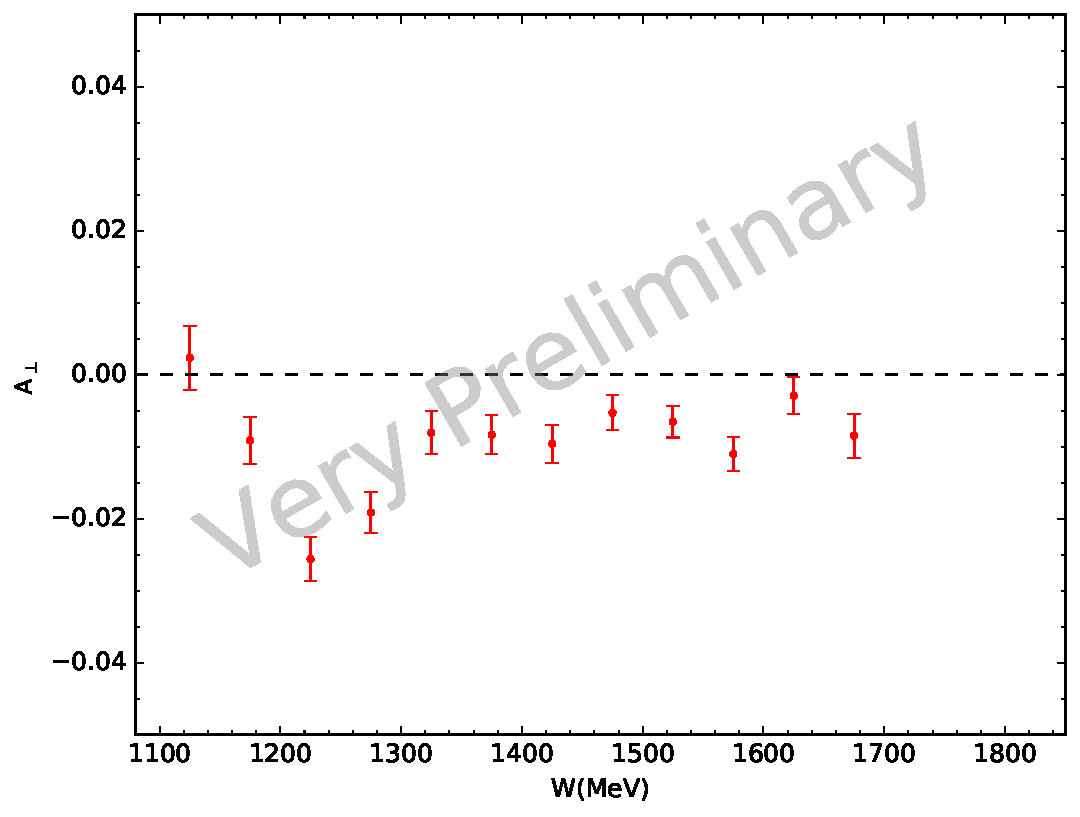
\includegraphics[width=0.79\textwidth]{figs/asymmetry-33505090.pdf}
  \caption[Physics asymmetries with $E=3.350$ GeV and $B=5.0$ T.]{Physics asymmetries for the configurations with 3.350 GeV beam energy and 5.0 T transverse target field. The uncertainties shown are only statistical. \label{C8S1F4}}
\end{figure}

The statistical uncertainties of the physics asymmetries are shown in the plots. If we assume the total event amount is $N\approx2N^+\approx2N^-$, the absolute statistical uncertainty of the asymmetries is $\sim1/\sqrt{N}$. This statement is valid because the fluctuations of the event amount $N^{\pm}$ follow the Poisson distribution, which are $\Delta N^{\pm}\equiv\sqrt{N^{\pm}}$ here. However, the DAQ event rate is reduced by applying a prescale factor $ps$ when the raw trigger rate is high. In this case, the fluctuations of the event amount $\Delta N$ no longer follow the Poisson distribution, and need to be corrected by a factor $S$ \cite{Qiang2007}:
\begin{equation} \label{C8S1E1}
S = \sqrt{1-LT\cdot f_A(1-\frac{1}{ps})},
\end{equation}
where $LT$ is the livetime correction of the DAQ system and $f_A$ is the acceptance correction which is defined as $f_A=N_{\mathrm{accepted}}/N_{\mathrm{total}}$. The statistical uncertainty can then be written as:
\begin{equation} \label{C8S1E2}
\delta A \simeq \frac{1}{2}\sqrt{\frac{S_+^2}{N_+}+\frac{S_-^2}{N_-}}.
\end{equation}

During the experiment, the data is taken in ``runs'', each containing about 7 million events. \cref{C8S1E2} can be used to calculate the uncertainty for each run, and the final asymmetry must be combined using a statistically weighted average:
\begin{equation} \label{C8S1E3}
A = \frac{\sum_iA_i/\delta A_i^2}{\sum_i1/\delta A_i^2},
\end{equation}
\begin{equation} \label{C8S1E4}
\delta A = \sqrt{\frac{1}{\sum_i1/\delta A_i^2}},
\end{equation}
where $A_i$ is the asymmetry calculated for the $i$th run, $\delta A_i$ is the statistical uncertainty given by \cref{C8S1E2}, and the summation is over all runs.

\section{Radiative Corrections}
\label{C8S2}

The Feynman diagram shown in \Cref{C2S1F1} only considers the leading order process, which is known as the Born approximation. This is assumed for theoretical analyses of lepton-nucleon scattering. However, the data contains all of the high order effects which need to be corrected for the data to be compared with theoretical results. This correction is referred to as the radiative correction.

The radiative correction arises from several different sources. The virtual photon one-loop corrections are shown in \Cref{C8S2F1}. It includes (a) the vacuum polarization correction where the virtual photon splits into an $e^-/e^+$ pair and acts as an electric dipole, (b) the vertex correction, (c)(d) the electron self-energy which contribute to the renormalization of the electron mass and (e)(f) the Bremsstrahlung radiation.

\begin{figure}[tb!]
  \centering
  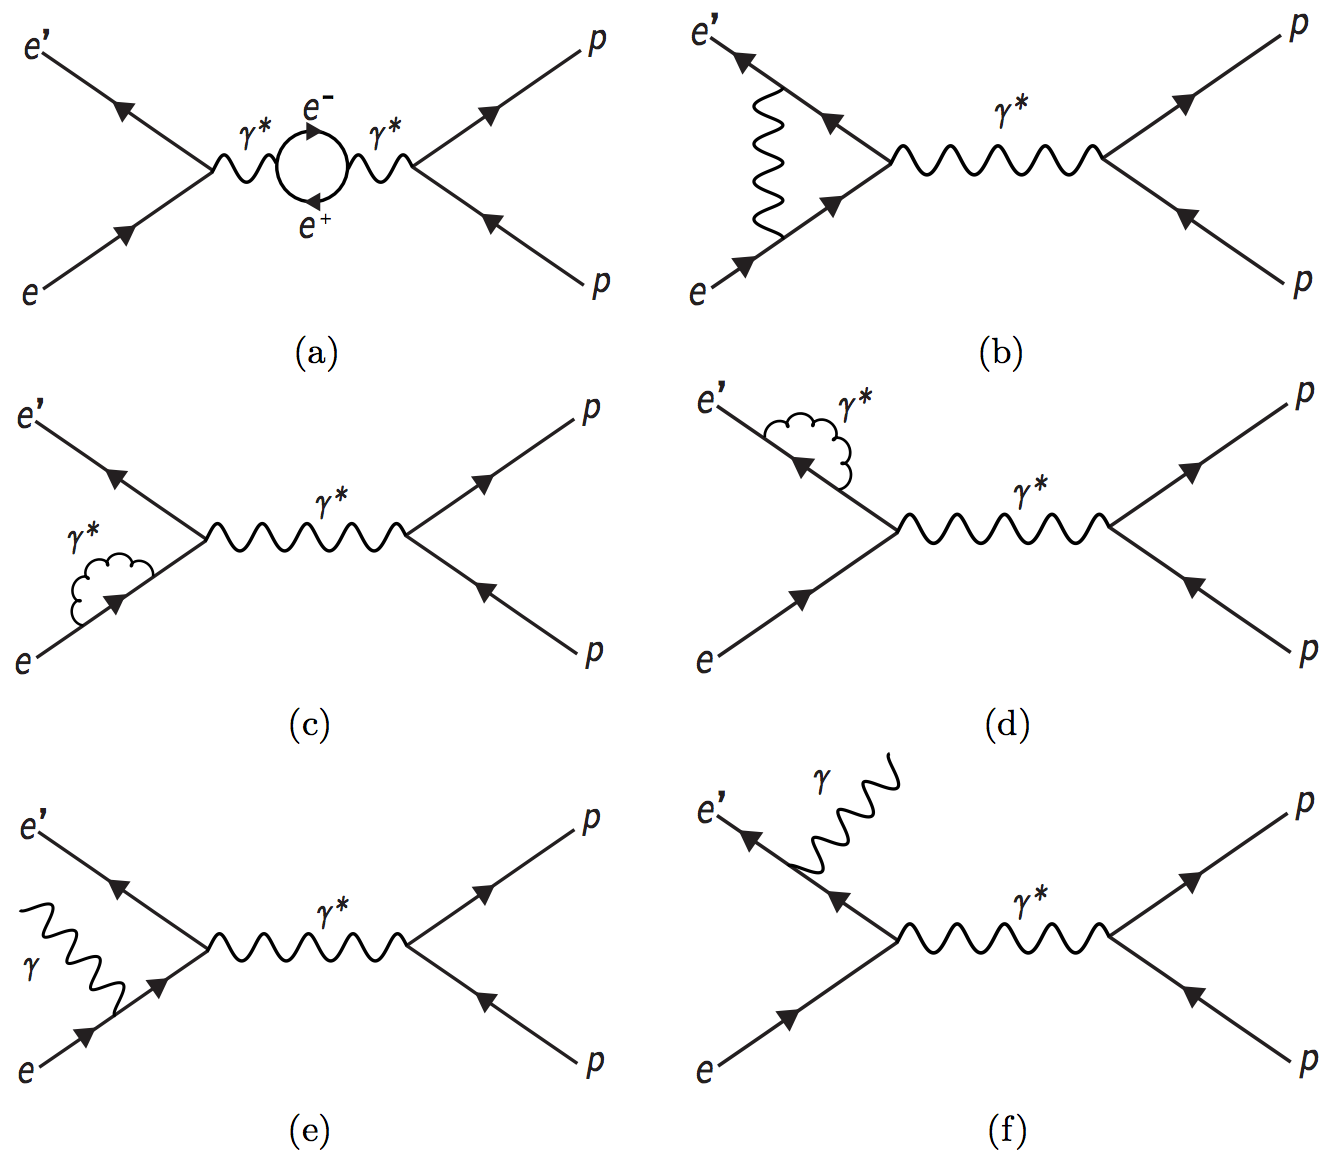
\includegraphics[width=0.75\textwidth]{figs/one-loop-corrections.png}
  \caption[Diagrams for next-to-leading order corrections.]{Diagrams for next-to-leading order corrections. Plot reproduced from \cite{Zielinski2014b}. \label{C8S2F1}}
\end{figure}

Diagrams (a), (b), (c) and (d) are considered to be relatively small compared to the contributions of the internal and external Bremsstrahlung. The internal Bremsstrahlung happens when the electron emits and re-absorbs a photon due to effect from the target nucleon's field, whereas the external Bremsstrahlung happens when the electron passes through the materials before or after the interaction. In addition to the Bremsstrahlung, energy can also be lost when an electron passes through the materials, due to ionization effect. The ionization energy loss is dependent on the radiation thickness of the material the electron passes through. The ionization energy loss is typically in the order of a few MeVs for the targets in this experiment.

The radiative corrections should be applied to the asymmetry and the cross-section results extracted from the data. For preliminary study, the asymmetry results from data were not radiatively corrected, but they are compared with radiative corrected model predictions. The Mainz online partial-wave analysis of meson electroproduction (MAID model) \cite{Drechsel2007} is used to generate the polarized cross-section differences. The radiative effects are separated into the internal part and the external part for convenience. The POLRAD formalism \cite{Akushevich1997} is used to calculate the internal radiative effects. And the methods in Ref. \cite{Mo1969} developed by Mo and Tsai is used to evaluate the external radiative effects.

The fits of P. Bosted to the inclusive inelastic electron scattering \cite{Bosted2008} are used to generate the unpolarized cross-sections, which also need to be corrected by the radiative effects. The radiative effects are calculated using the same formalism as the polarized cross-section differences with the fits of P. Bosted as input for both the internal and external corrections.

The elastic tail must also be considered since it becomes significant in the resonance region. The MASCARD code \cite{Afanasev2001} is used to generate polarized elastic cross-sections. And the form factors from Mo and Tsai are used to calculate the radiative effects for both the polarized and unpolarized radiative effects.

\begin{figure}[tb!]
  \centering
  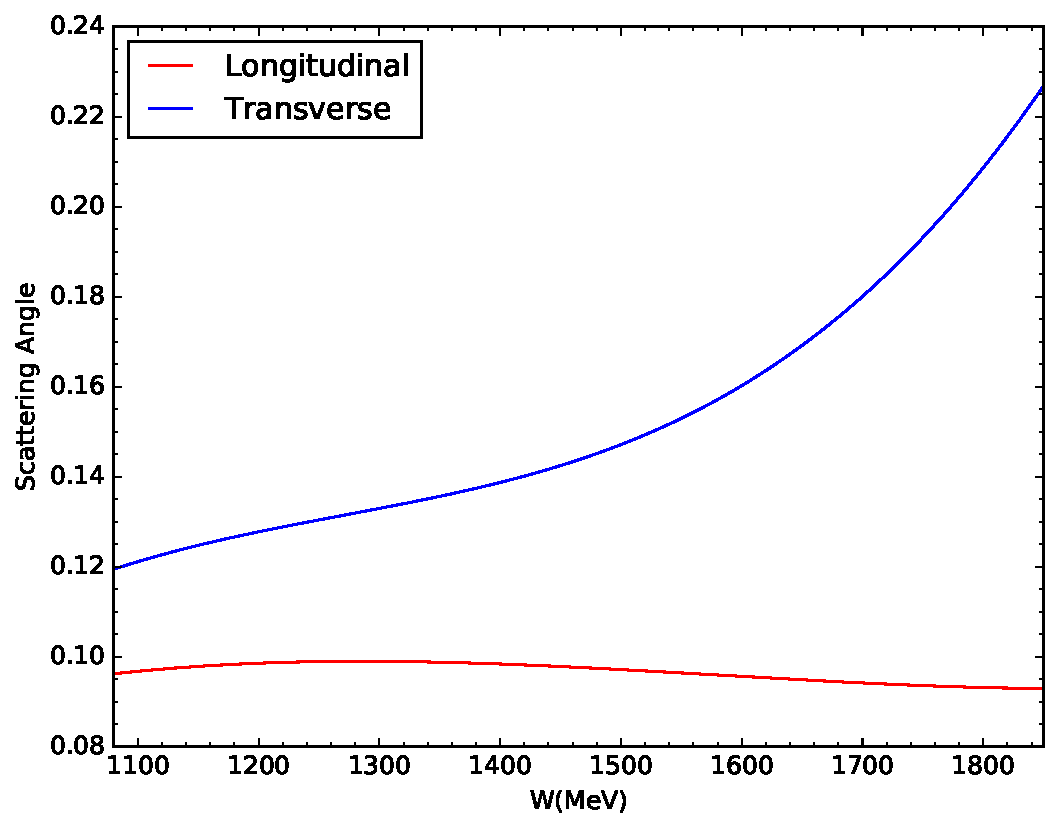
\includegraphics[width=0.6\textwidth]{figs/scattering-angle.pdf}
  \caption[Relations between the scattering angle and $W$.]{Relations between the scattering angle and $W$ for the kinematic settings with 2.253 GeV beam energy and 5.0 T target field (longitudinal and transverse configuration). \label{C8S2F2}}
\end{figure}

To account for the actual kinematic coverage in the calculation, the data are used to provide a fit of the relation between the scattering angle and $W$ for each kinematic setting, and the $Q^2$ can be determined with $W$ and the scattering angle. The value of $W$ and the $Q^2$, $\theta$ values from the fit are used in the model as inputs. \Cref{C8S2F2} shows the relations between $W$ and the scattering angle. Only the two settings with 2.253 GeV beam energy and 5.0 T target field are shown in the figure as examples. The variation of the scattering angle is an effect of the target magnetic field. As shown in \Cref{C8S2F2}, the variation is very small for the longitudinal configuration but for transverse configuration it is significant. The radiated and unradiated model predictions for the asymmetries are compared in \Cref{C8S2F3}. Here only the two kinematic settings (longitudinal and transverse configurations) with 2.253 GeV beam energy and 5.0 T target field are shown as examples.

\begin{figure}[p!]
  \centering
  \begin{subfigure}[t]{0.79\textwidth}
    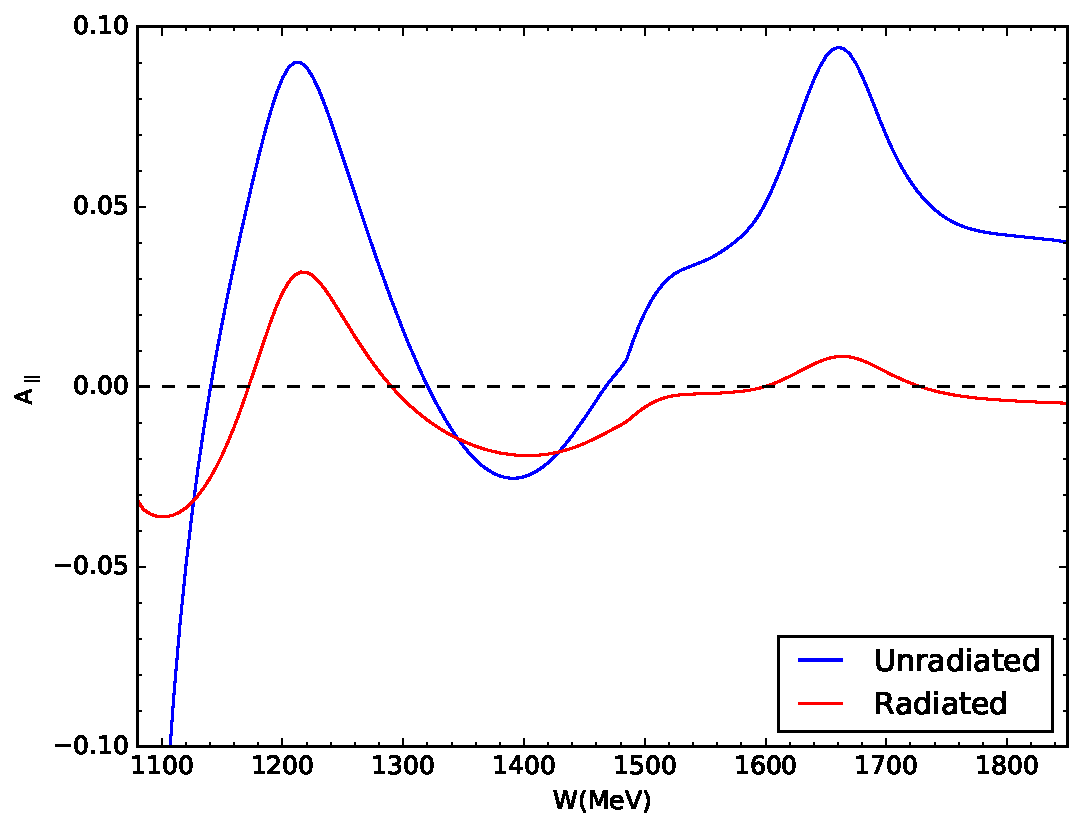
\includegraphics[width=\textwidth]{figs/asymmetry-model-22535000.pdf}
    \caption{Longitudinal configuration. \label{C8S2F3a}}
  \end{subfigure}
  \begin{subfigure}[t]{0.79\textwidth}
    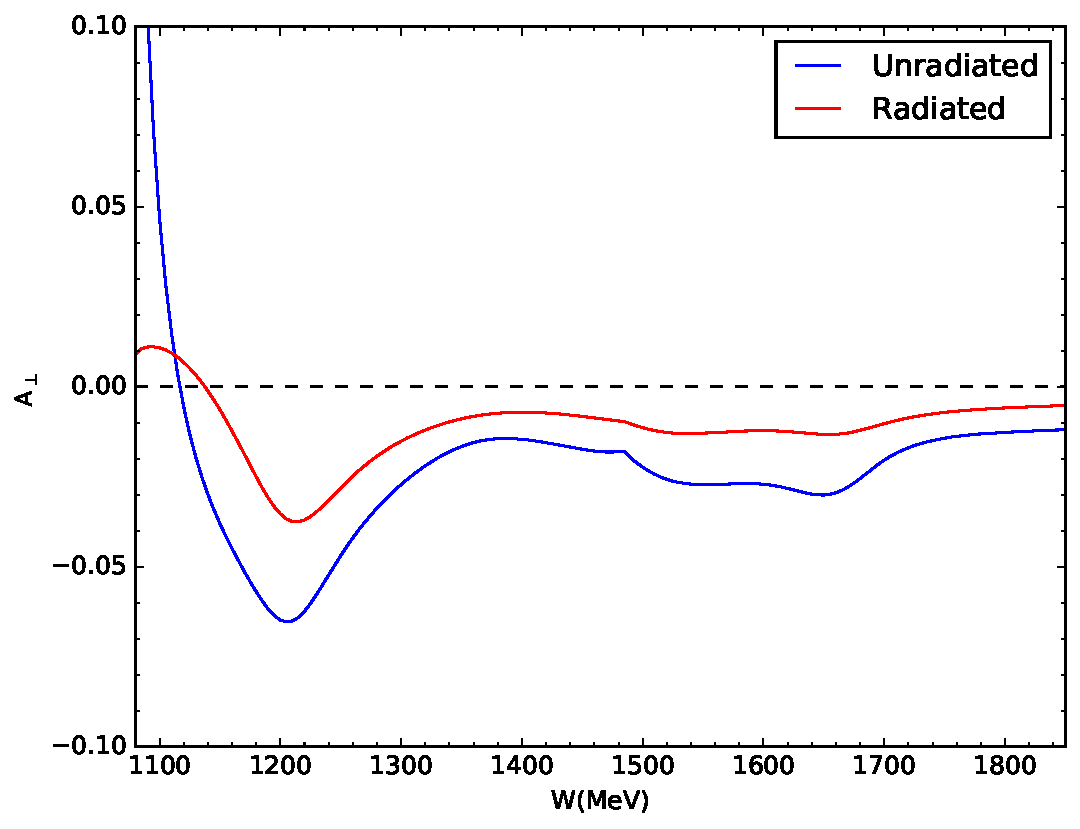
\includegraphics[width=\textwidth]{figs/asymmetry-model-22535090.pdf}
    \caption{Transverse configuration. \label{C8S2F3b}}
  \end{subfigure}
  \caption[Comparison of the radiated and unradiated model predictions.]{Comparison of the radiated and unradiated model predictions for the asymmetries of the kinematic setting with 2.253 GeV beam energy and 5.0 T target field. \label{C8S2F3}}
\end{figure}

\begin{figure}[p!]
  \centering
  \begin{subfigure}[t]{0.79\textwidth}
    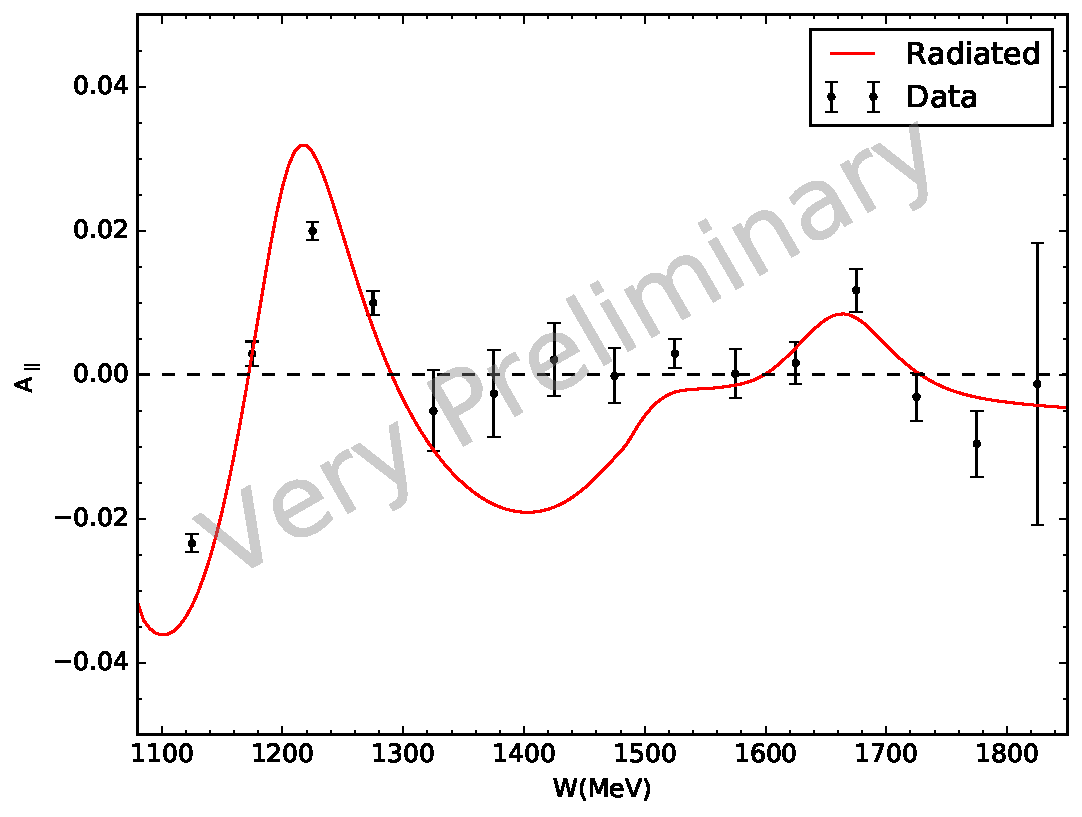
\includegraphics[width=\textwidth]{figs/asymmetry-data-model-22535000.pdf}
    \caption{Longitudinal configuration. \label{C8S2F4a}}
  \end{subfigure}
  \begin{subfigure}[t]{0.79\textwidth}
    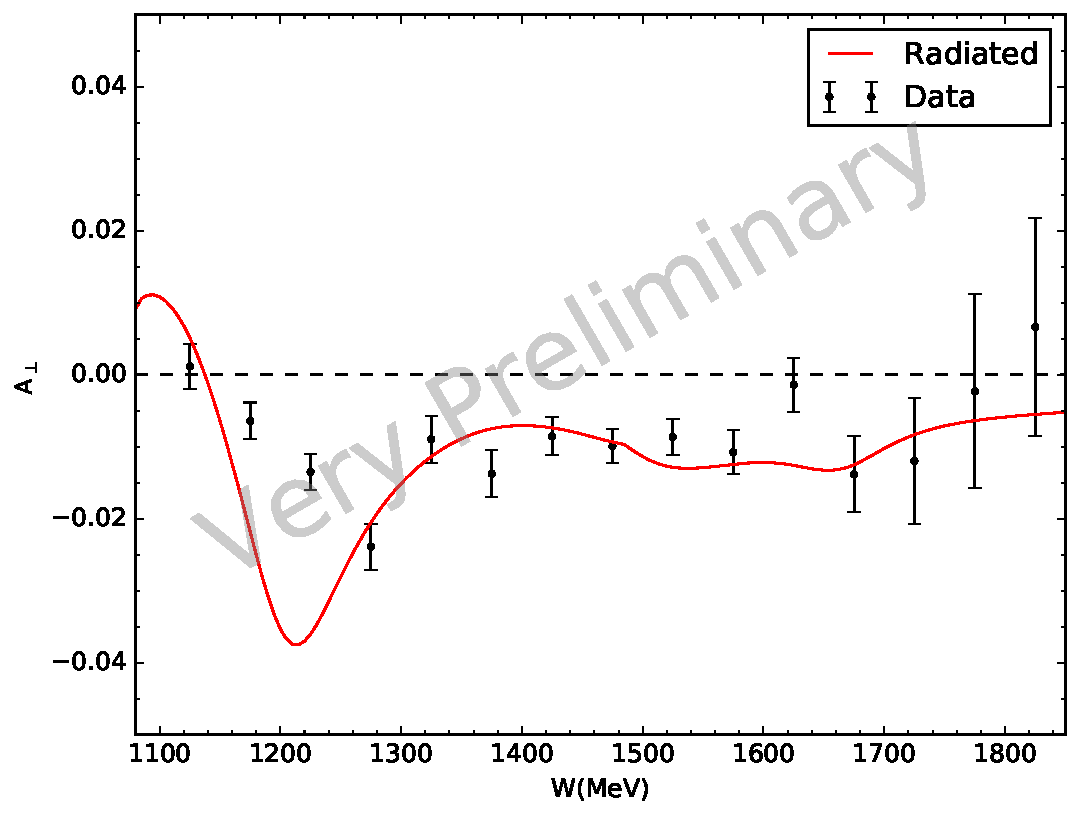
\includegraphics[width=\textwidth]{figs/asymmetry-data-model-22535090.pdf}
    \caption{Transverse configuration. \label{C8S2F4b}}
  \end{subfigure}
  \caption[Asymmetries with $E=2.253$ GeV and $B=5.0$ T.]{Comparison of the radiated model predictions with measured asymmetries for the kinematic settings with 2.253 GeV beam energy and 5.0 T target field (longitudinal and transverse configurations). Data are not radiatively corrected. \label{C8S2F4}}
\end{figure}

\begin{figure}[p!]
  \centering
  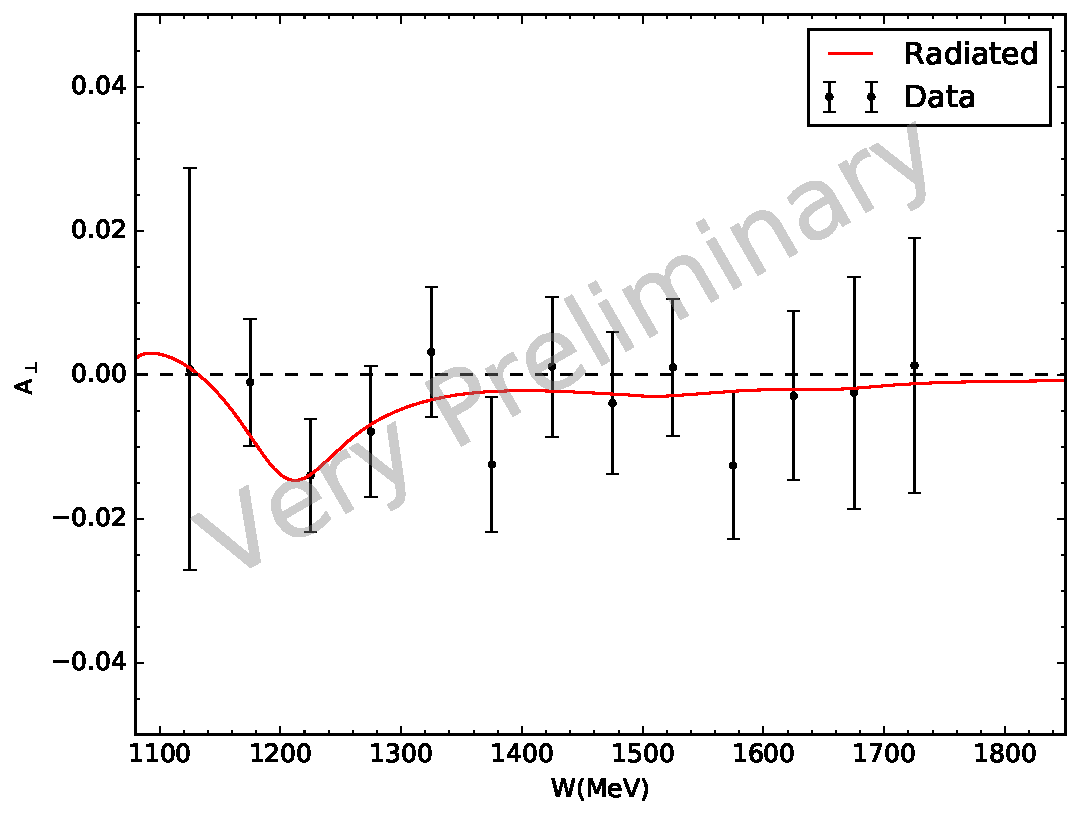
\includegraphics[width=0.79\textwidth]{figs/asymmetry-data-model-17102590.pdf}
  \caption[Asymmetries with $E=1.710$ GeV and $B=2.5$ T.]{Comparison of the radiated model predictions with measured asymmetries for the kinematic settings with 1.710 GeV beam energy and 2.5 T transverse target field. Data are not radiatively corrected. \label{C8S2F5}}
\end{figure}

\begin{figure}[p!]
  \centering
  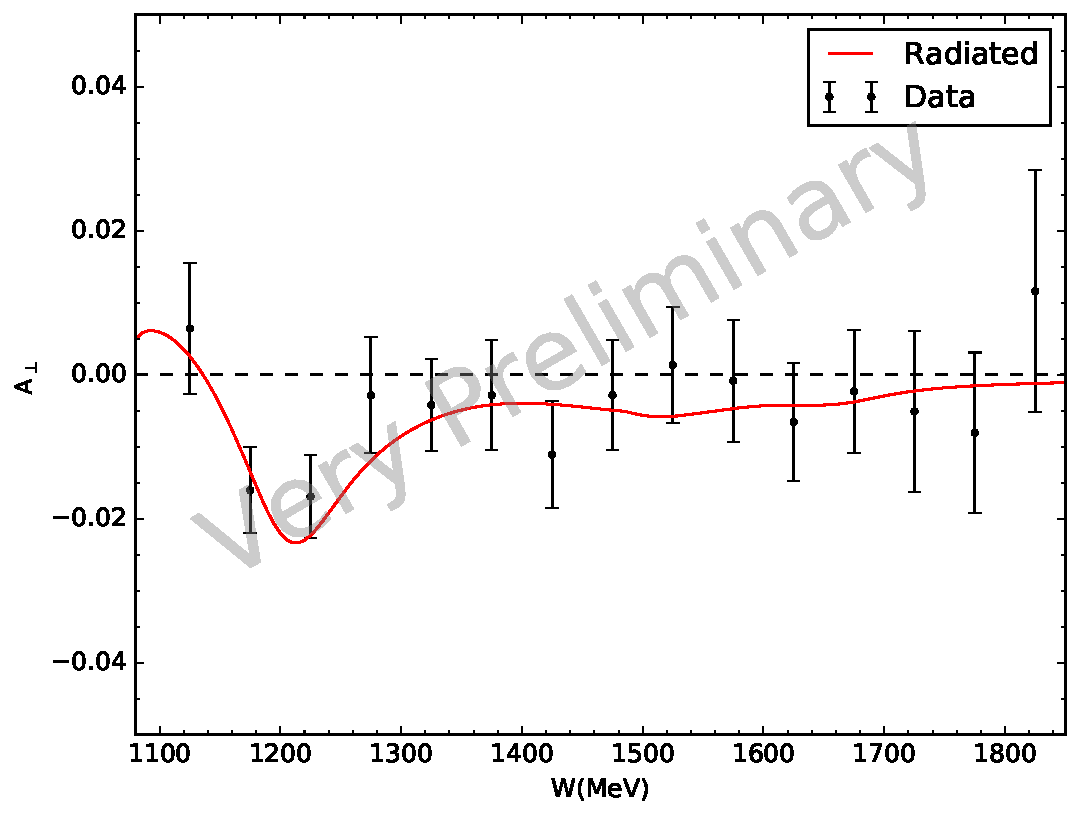
\includegraphics[width=0.79\textwidth]{figs/asymmetry-data-model-22532590.pdf}
  \caption[Asymmetries with $E=2.253$ GeV and $B=2.5$ T.]{Comparison of the radiated model predictions with measured asymmetries for the kinematic settings with 2.253 GeV beam energy and 2.5 T transverse target field. Data are not radiatively corrected. \label{C8S2F6}}
\end{figure}

\begin{figure}[tb!]
  \centering
  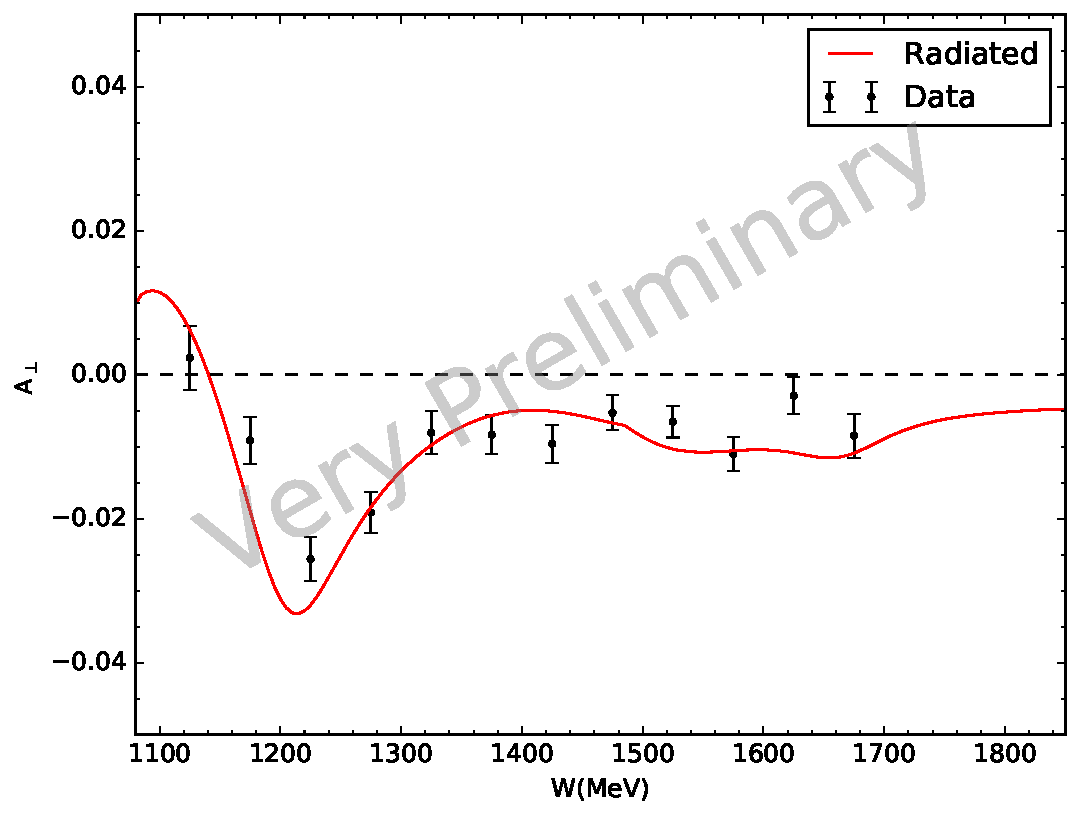
\includegraphics[width=0.79\textwidth]{figs/asymmetry-data-model-33505090.pdf}
  \caption[Asymmetries with $E=3.350$ GeV and $B=5.0$ T.]{Comparison of the radiated model predictions with measured asymmetries for the kinematic settings with 3.350 GeV beam energy and 5.0 T transverse target field. Data are not radiatively corrected. \label{C8S2F7}}
\end{figure}

\Cref{C8S2F4,C8S2F5,C8S2F6,C8S2F7} shows the comparison of the radiated model predictions with the physics asymmetries extracted in the previous section. There can be an uncertainty for the model prediction, which arises from several different sources. The fits of P. Bosted contribute a relative uncertainty of 5\% \cite{Bosted2008} and the Mo and Tsai formalism contributes a relative uncertainty of 4\% \cite{Mo1969}. The MAID group does not provide the fit uncertainties since the fit uncertainty is unrealistically small in this case due to the large number of data points included in the fit. Thus, we will use the difference between the model prediction and our data as the uncertainty of the model when we calculate the cross-section differences in the next section. The acceptance effects also contribute to the uncertainty when we fit the relationship between $W$ and the scattering angle with data. Since the acceptance analysis is still on-going, its contribution to the uncertainty of the model prediction has not been determined yet.

\section{Polarized Cross-Section Differences}
\label{C8S3}

The polarized cross-section differences can be calculated via \cref{C7S1E7}. The asymmetries $A_{\parallel,\perp}$ were presented in the previous section. Since the acceptance analysis is still on-going, the unpolarized cross-sections extracted from our data are not reliable yet. Thus, the fits of P. Bosted \cite{Bosted2008} are used for the unpolarized cross-section as inputs to \cref{C7S1E7} to extract $\Delta\sigma_{\parallel,\perp}$.

In order to extract the polarized structure functions, the cross-section differences need to be radiative corrected. The standard method to perform radiative correction is to deconvolute the spectrum extracted from the data with the help of a simulation. In this thesis, we perform the radiative correction to the asymmetries in an alternate way. If we denote the radiated and unradiated model predictions of asymmetries by $A_{\mathrm{rad}}^{\mathrm{model}}$ and $A_{\mathrm{unrad}}^{\mathrm{model}}$ respectively, the difference between the radiated and unradiated models can be expressed as:
\begin{equation} \label{C8S3E1}
\Delta_{\mathrm{RC}}^{\mathrm{model}} = A_{\mathrm{unrad}}^{\mathrm{model}}-A_{\mathrm{rad}}^{\mathrm{model}}.
\end{equation}
$\Delta_{\mathrm{RC}}^{\mathrm{model}}$ is taken as the radiative correction, and the asymmetries and the cross-section differences can be expressed as:
\begin{gather} \label{C8S3E2}
A_{\mathrm{corrected}} = A_{\mathrm{uncorrected}}-\Delta_{\mathrm{RC}}^{\mathrm{model}}, \\ \label{C8S3E3}
\Delta\sigma_{\parallel,\perp}^{\mathrm{corrected}} = 2A_{\parallel,\perp}^{\mathrm{corrected}} \cdot \sigma_0^{\mathrm{corrected}}.
\end{gather}

\begin{figure}[p!]
  \centering
  \begin{subfigure}[t]{0.79\textwidth}
    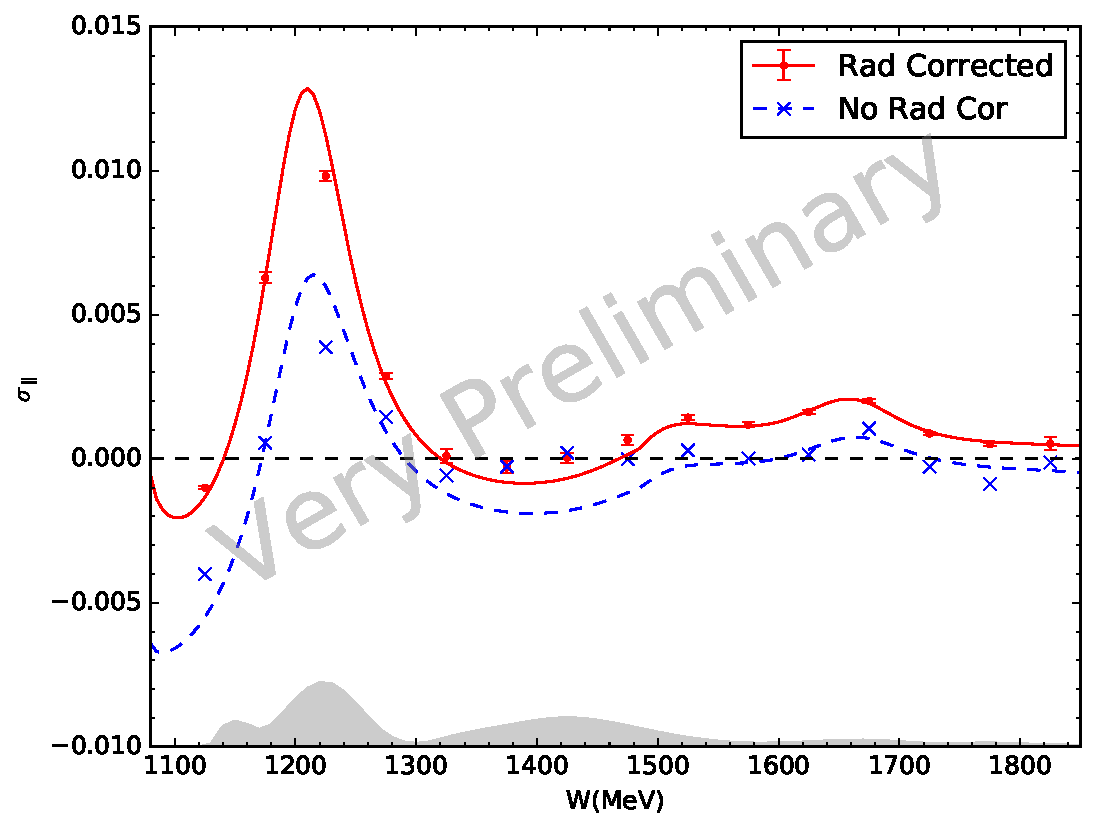
\includegraphics[width=\textwidth]{figs/xsdiff-model-22535000.pdf}
    \caption{Longitudinal configuration. \label{C8S3F1a}}
  \end{subfigure}
  \begin{subfigure}[t]{0.79\textwidth}
    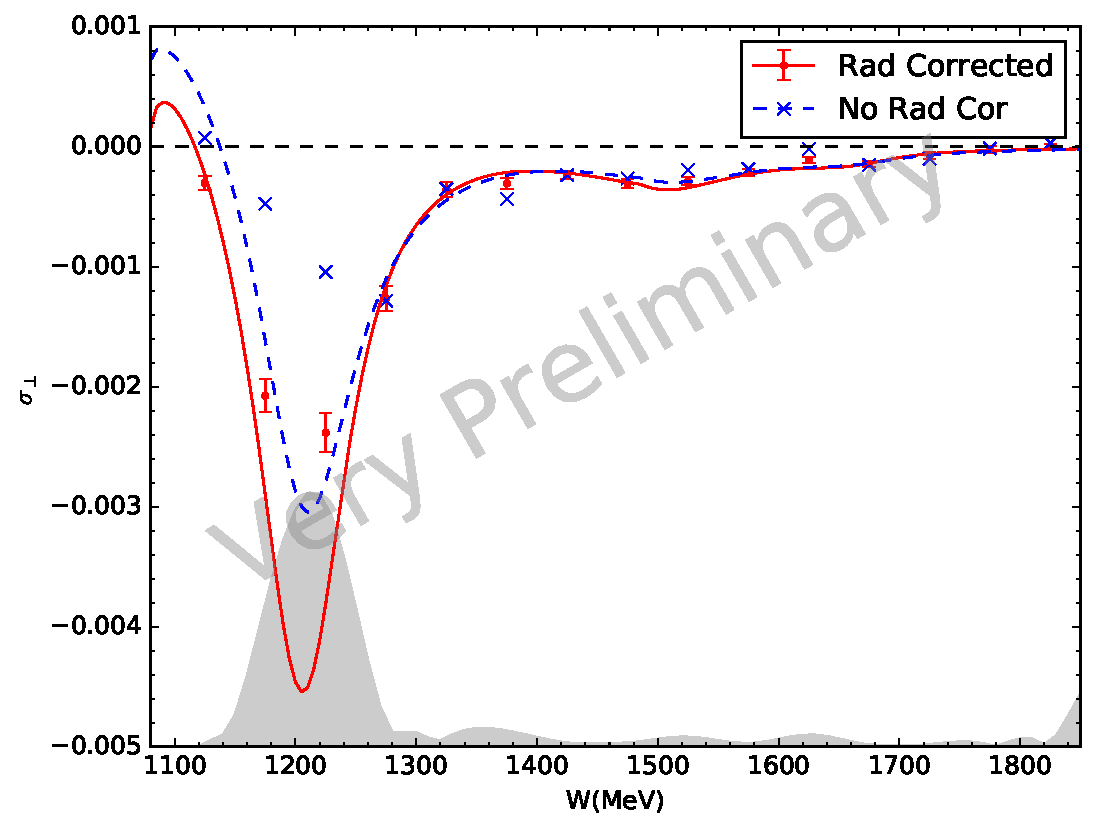
\includegraphics[width=\textwidth]{figs/xsdiff-model-22535090.pdf}
    \caption{Transverse configuration. \label{C8S3F1b}}
  \end{subfigure}
  \caption[Cross-section differences with $E=2.253$ GeV and $B=5.0$ T.]{Comparison of the radiative corrected and uncorrected cross-section differences for the kinematic settings with 2.253 GeV beam energy and 5.0 T target field (longitudinal and transverse configurations). The error bars for the uncorrected data are not shown in this plot. \label{C8S3F1}}
\end{figure}

\begin{figure}[p!]
  \centering
  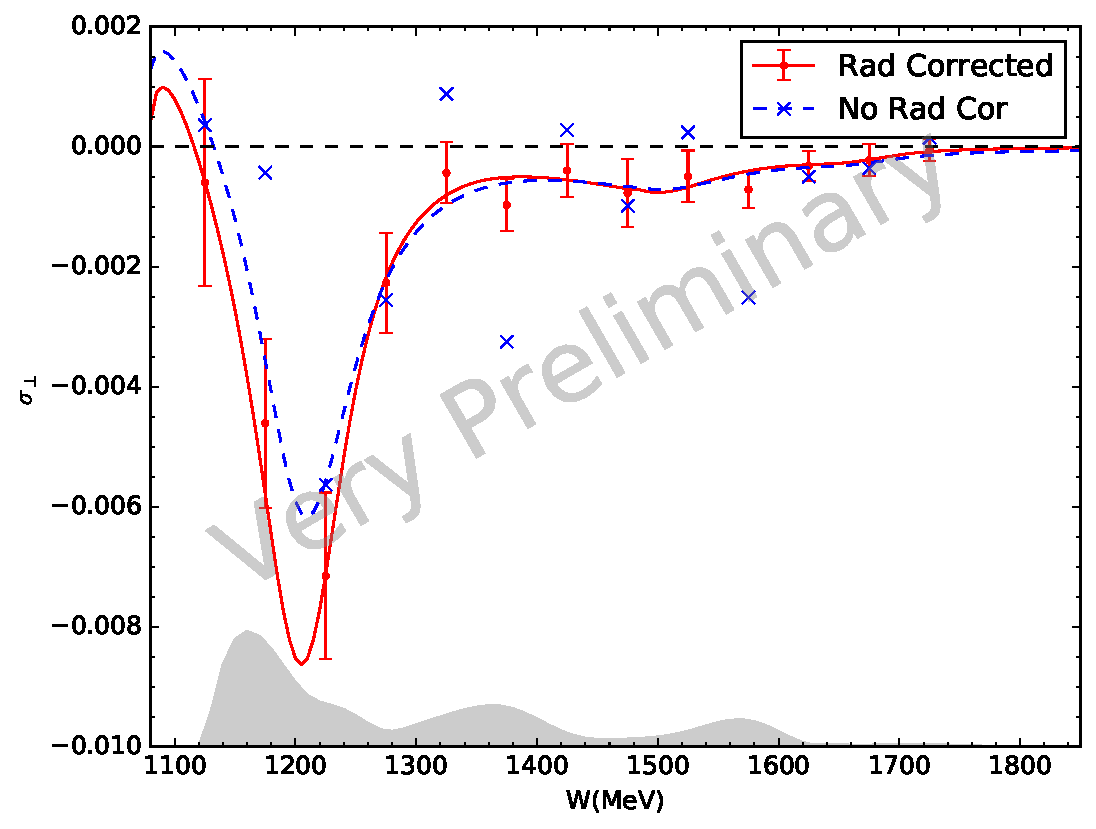
\includegraphics[width=0.79\textwidth]{figs/xsdiff-model-17102590.pdf}
  \caption[Cross-section differences with $E=1.710$ GeV and $B=2.5$ T.]{Comparison of the radiative corrected and uncorrected cross-section differences for the kinematic settings with 1.710 GeV beam energy and 2.5 T transverse target field. The error bars for the uncorrected data are not shown in this plot. \label{C8S3F2}}
\end{figure}

\begin{figure}[p!]
  \centering
  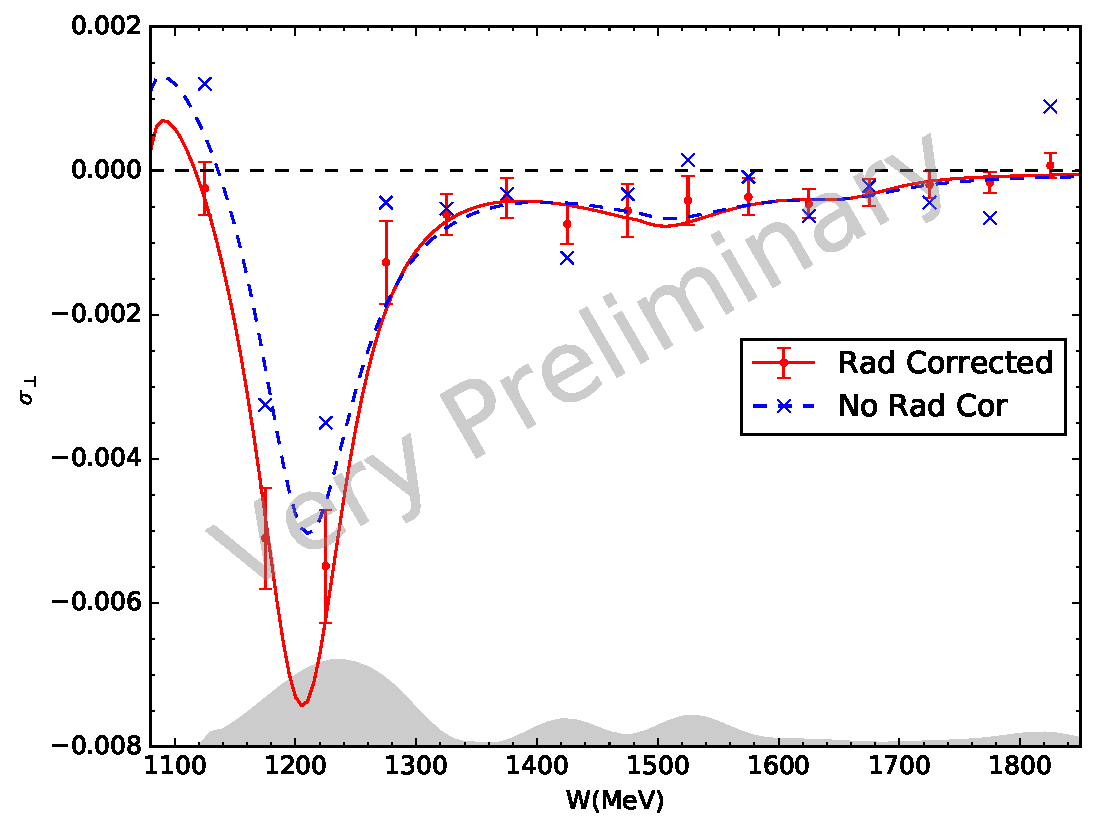
\includegraphics[width=0.79\textwidth]{figs/xsdiff-model-22532590.pdf}
  \caption[Cross-section differences with $E=2.253$ GeV and $B=2.5$ T.]{Comparison of the radiative corrected and uncorrected cross-section differences for the kinematic settings with 2.253 GeV beam energy and 2.5 T transverse target field. The error bars for the uncorrected data are not shown in this plot. \label{C8S3F3}}
\end{figure}

\begin{figure}[tb!]
  \centering
  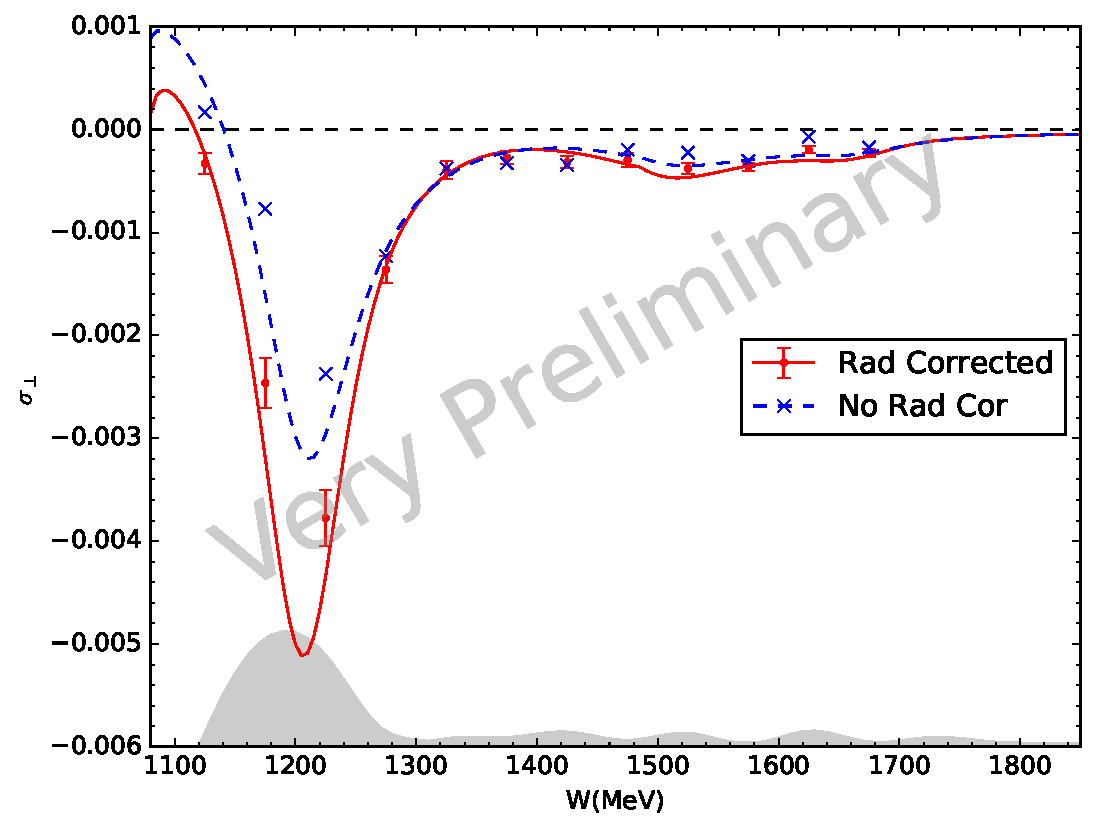
\includegraphics[width=0.79\textwidth]{figs/xsdiff-model-33505090.pdf}
  \caption[Cross-section differences with $E=3.350$ GeV and $B=5.0$ T.]{Comparison of the radiative corrected and uncorrected cross-section differences for the kinematic settings with 3.350 GeV beam energy and 5.0 T transverse target field. The error bars for the uncorrected data are not shown in this plot. \label{C8S3F4}}
\end{figure}

The radiative-corrected cross-section differences are shown in \Cref{C8S3F1,C8S3F2,C8S3F3,C8S3F4}. The radiated and unradiated model predictions of the cross-section differences are also shown in the figures for comparison. The error bars on each data point are statistical only.

The systematic uncertainty of these cross-section difference results has two major contributions: the systematic uncertainties of the asymmetries $A_{\parallel,\perp}$ and the unpolarized cross-sections $\sigma_0$. Since the unpolarized cross-sections are given by the fits of P. Bosted, the systematic uncertainties contributed by $\sigma_0$ are 5\%. There are several different contributions to the systematic uncertainty of the asymmetry results. The dilution factors are calculated from the packing fraction with \cref{C7S4E12}. The uncertainties of the packing fractions are listed in \Cref{C7S3T1} and there is an additional $\approx$5\% uncertainty to account for the fact that the dilution factors are extracted from calculated cross-sections using P. Bosted's fits. The uncertainties of the beam polarization and the target polarization are $\approx$1.7\% and $\approx$1.2\% respectively, which have been described in \Cref{C5}. The largest contribution to the uncertainty comes from the models we used to perform the radiative correction. As mentioned in \Cref{C8S2}, the difference between the MAID model and our data is taken as the uncertainty in the analysis. Thus, we could combine all of these contributions to estimate the systematic uncertainty of the cross-section differences. The estimations of the systematic uncertainty are shown as the grey bands in \Cref{C8S3F1,C8S3F2,C8S3F3,C8S3F4}.

\section{\texorpdfstring{Spin Structure Function $g_2^p$}{Spin Structure Function g2p}}
\label{C8S4}

\begin{figure}[p!]
  \centering
  \begin{subfigure}[t]{0.79\textwidth}
    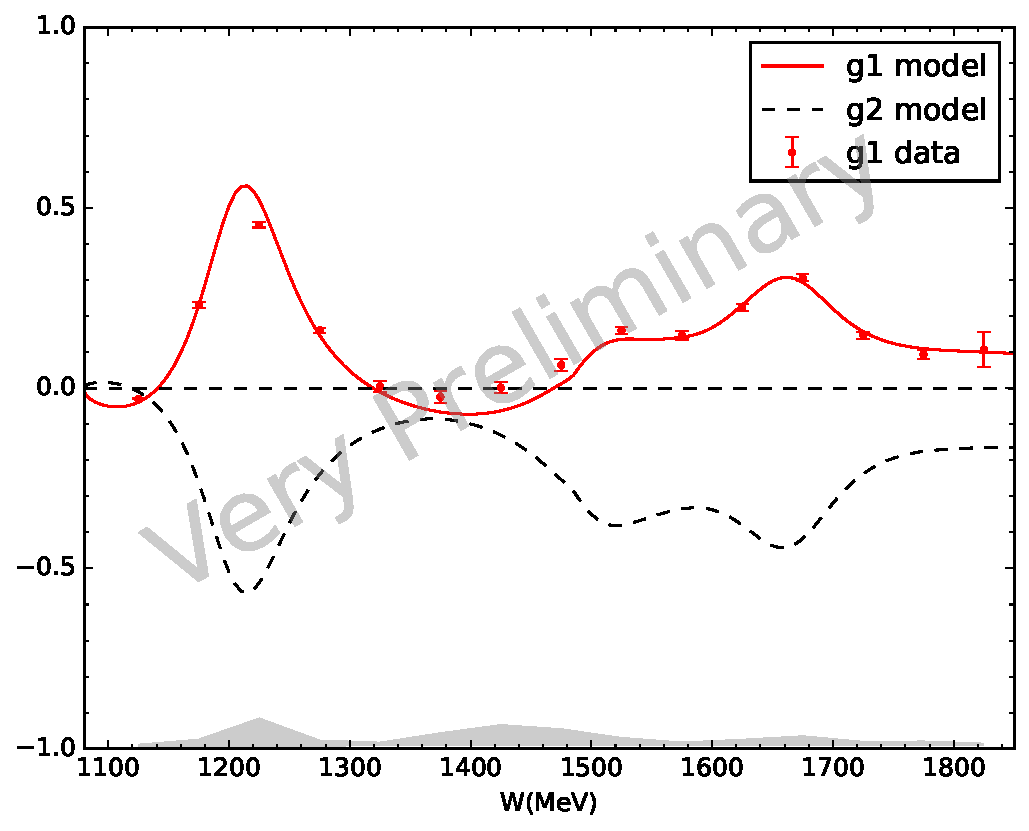
\includegraphics[width=\textwidth]{figs/g1g2-model-22535000.pdf}
    \caption{Longitudinal configuration. \label{C8S4F1a}}
  \end{subfigure}
  \begin{subfigure}[t]{0.79\textwidth}
    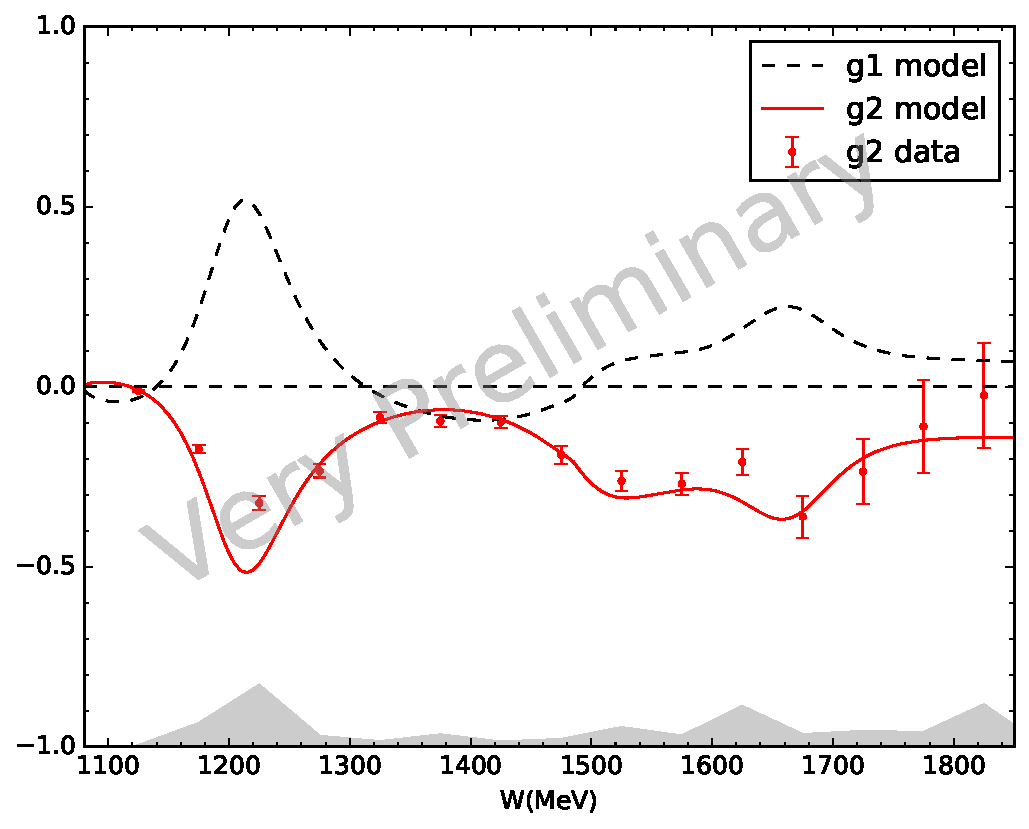
\includegraphics[width=\textwidth]{figs/g1g2-model-22535090.pdf}
    \caption{Transverse configuration. \label{C8S4F1b}}
  \end{subfigure}
  \caption[$g_1$ and $g_2$ results with $E=2.253$ GeV and $B=5.0$ T.]{$g_1$ and $g_2$ results for the kinematic settings with 2.253 GeV beam energy and 5.0 T target field (longitudinal and transverse configurations). The error bars on each data point are statistical. \label{C8S4F1}}
\end{figure}

\begin{figure}[p!]
  \centering
  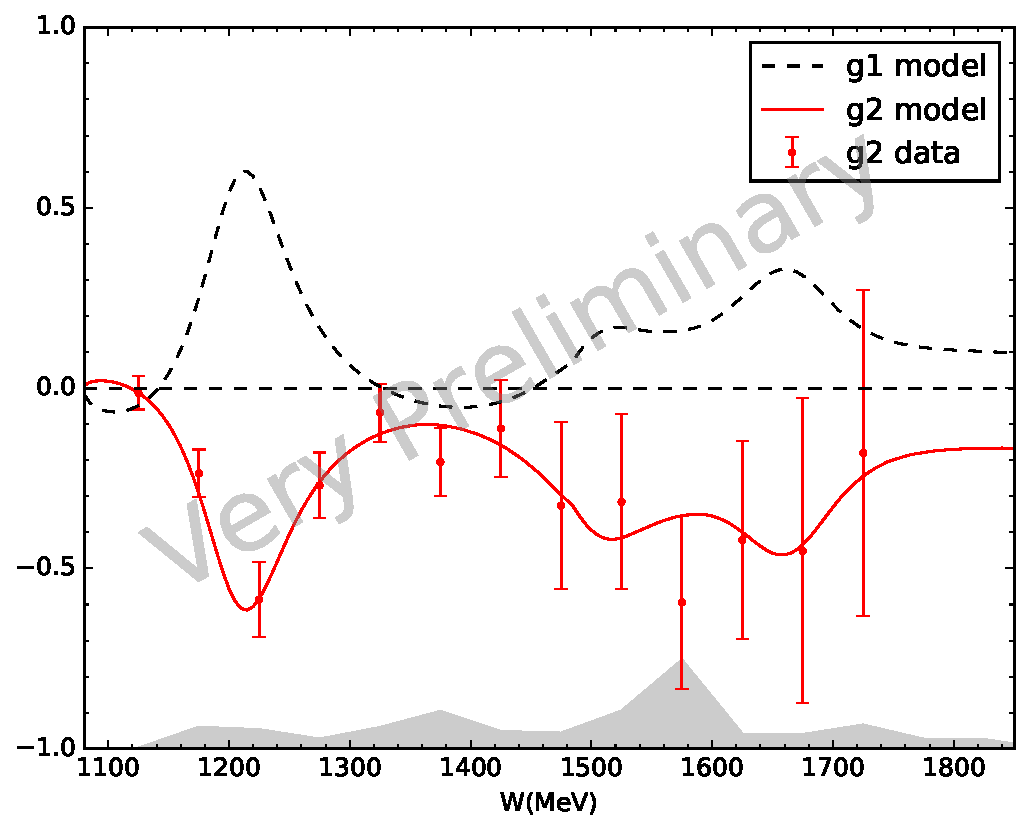
\includegraphics[width=0.79\textwidth]{figs/g1g2-model-17102590.pdf}
  \caption[$g_2$ results with $E=1.710$ GeV and $B=2.5$ T.]{$g_2$ results for the kinematic settings with 1.710 GeV beam energy and 2.5 T target field. The error bars on each data point are statistical. \label{C8S4F2}}
\end{figure}

\begin{figure}[p!]
  \centering
  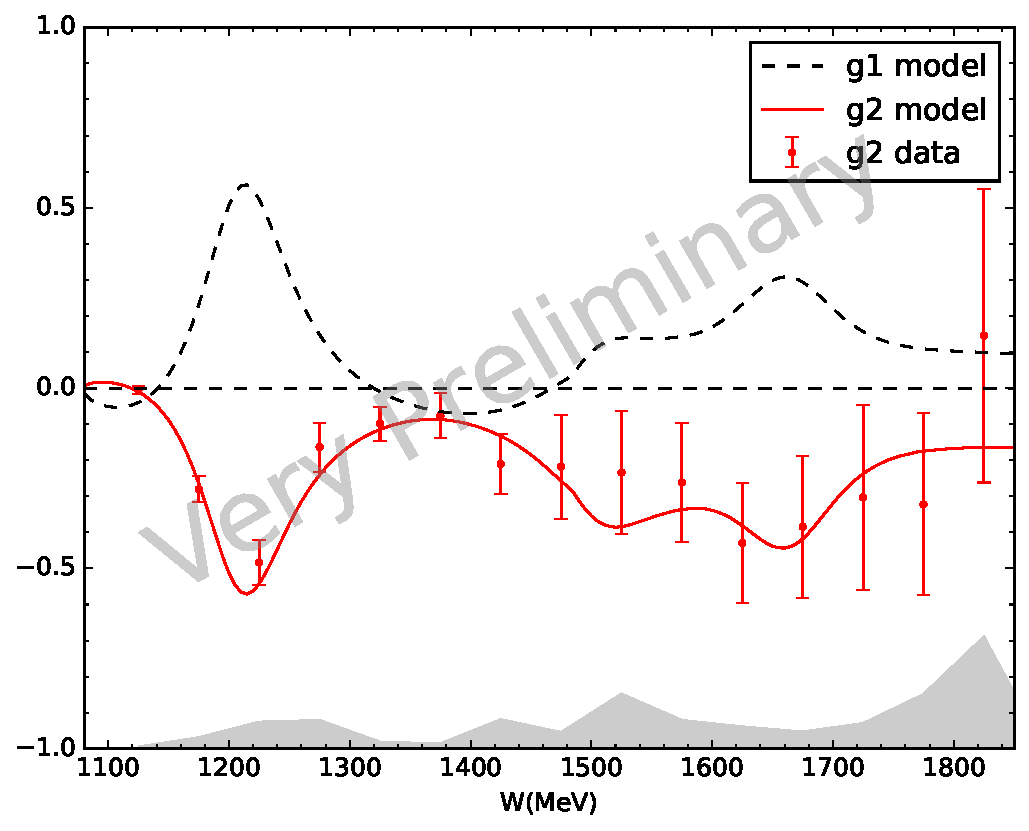
\includegraphics[width=0.79\textwidth]{figs/g1g2-model-22532590.pdf}
  \caption[$g_2$ results with $E=2.253$ GeV and $B=2.5$ T.]{$g_2$ results for the kinematic settings with 2.253 GeV beam energy and 2.5 T target field. The error bars on each data point are statistical. \label{C8S4F3}}
\end{figure}

\begin{figure}[tb!]
  \centering
  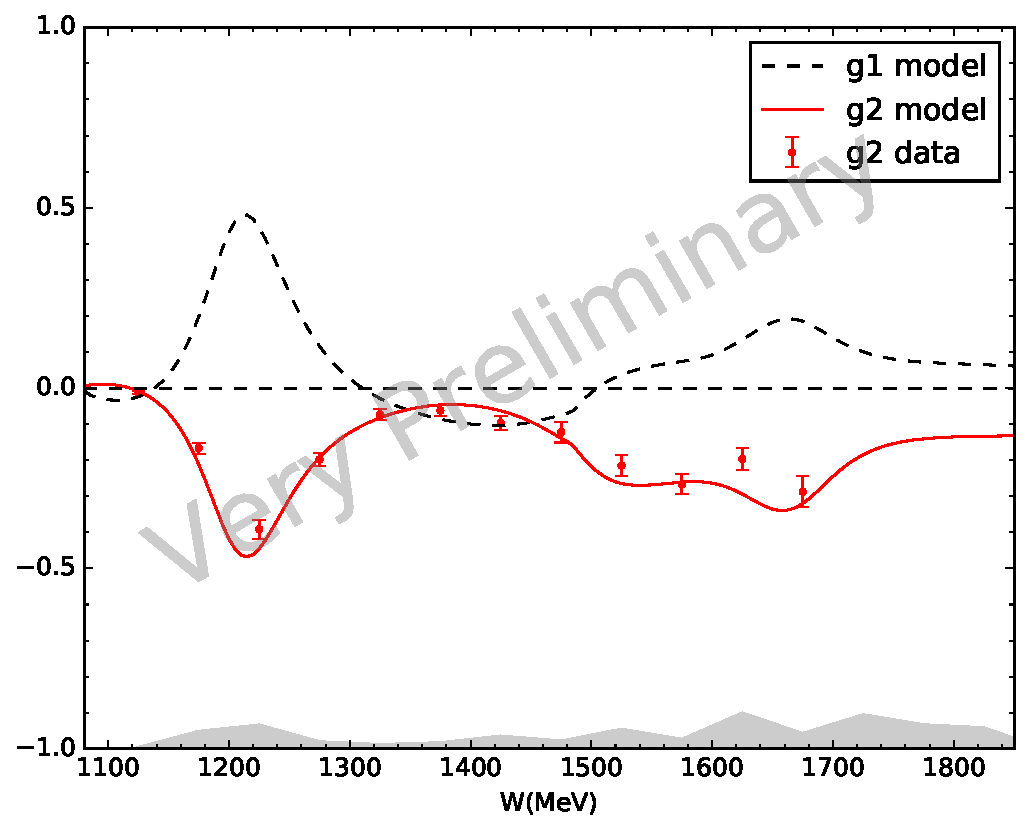
\includegraphics[width=0.79\textwidth]{figs/g1g2-model-33505090.pdf}
  \caption[$g_2$ results with $E=3.350$ GeV and $B=5.0$ T.]{$g_2$ results for the kinematic settings with 3.350 GeV beam energy and 5.0 T target field. The error bars on each data point are statistical. \label{C8S4F4}}
\end{figure}

In \Cref{C2S2}, we have derived the relationships between the polarized cross-section differences and the polarized structure functions \cref{C2S2E25,C2S2E26}. Thus, the polarized structure functions $g_1$ and $g_2$ can be written in terms of the cross-section differences as:
\begin{align} \label{C8S4E1}
g_1 & = \frac{MQ^2}{4\alpha^2}\frac{y}{(1-y)(2-y)}\left[\Delta\sigma_\parallel+\tan\frac{\theta}{2}\Delta\sigma_\perp\right], \\ \label{C8S4E2}
g_2 & = \frac{MQ^2}{4\alpha^2}\frac{y^2}{2(1-y)(2-y)}\left[-\Delta\sigma_\parallel+\frac{1+(1-y)\cos\theta}{(1-y)\sin\theta}\Delta\sigma_\perp\right],
\end{align}
where $y=\nu/E$.

For the preliminary results presented here, the results on $\Delta\sigma_\perp$ from \Cref{C8S2} were combined with model predictions of $\Delta\sigma_\parallel$ to extract $g_1$ and $g_2$ using \cref{C8S4E1,C8S4E2}. In addition, as described in \Cref{C8S2}, the $\Delta\sigma_\perp$ results were obtained using asymmetries measured in E08-027 combined with model predictions for $\sigma_0$. For the final analysis to be carried out in the future, $\Delta\sigma_\parallel$ will be replaced by the data form Jefferson Lab EG4 and $\Delta\sigma_\perp$ itself will be extracted from E08-027, thus completely eliminating the use of model predictions. For the kinematic setting with 2.253 GeV beam energy and 5.0 T target field, although both $\Delta\sigma_\perp$ and $\Delta\sigma_\parallel$ were measured during the experiment, the kinematics of the longitudinal and transverse configurations are not the same as shown in \Cref{C8S2F2}. Thus the model predictions for $\Delta\sigma_\parallel$ are also used in these settings. Results for $g_1$ and $g_2$ are shown in \Cref{C8S4F1,C8S4F2,C8S4F3,C8S4F4}. The systematic uncertainties are shown as the grey bands in the plots which contain the contributions from the systematic uncertainties of the transverse cross-section differences discussed in the previous section.

\section{\texorpdfstring{Spin Polarizability $\dlt$}{Spin Polarizability delta\_\{LT\}}}
\label{C8S5}

\begin{figure}[p!]
  \centering
  \begin{subfigure}[t]{0.79\textwidth}
    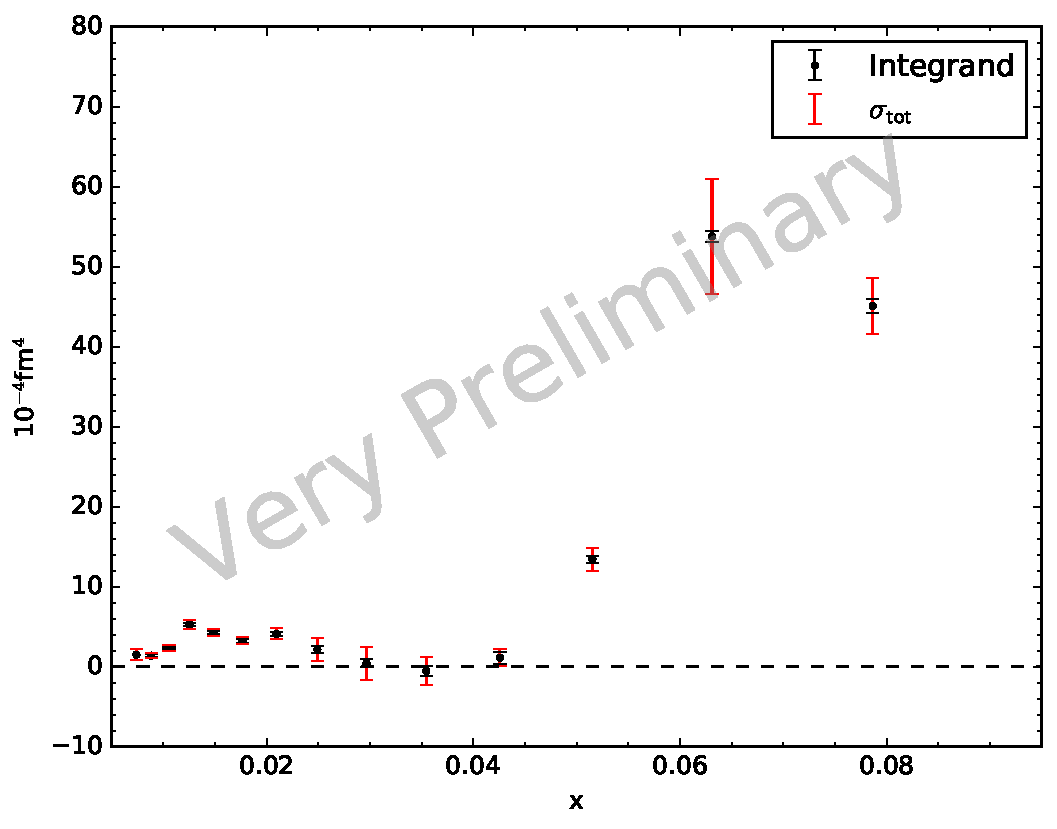
\includegraphics[width=\textwidth]{figs/gamma0-model-22535000.pdf}
    \caption{Longitudinal configuration. \label{C8S5F1a}}
  \end{subfigure}
  \begin{subfigure}[t]{0.79\textwidth}
    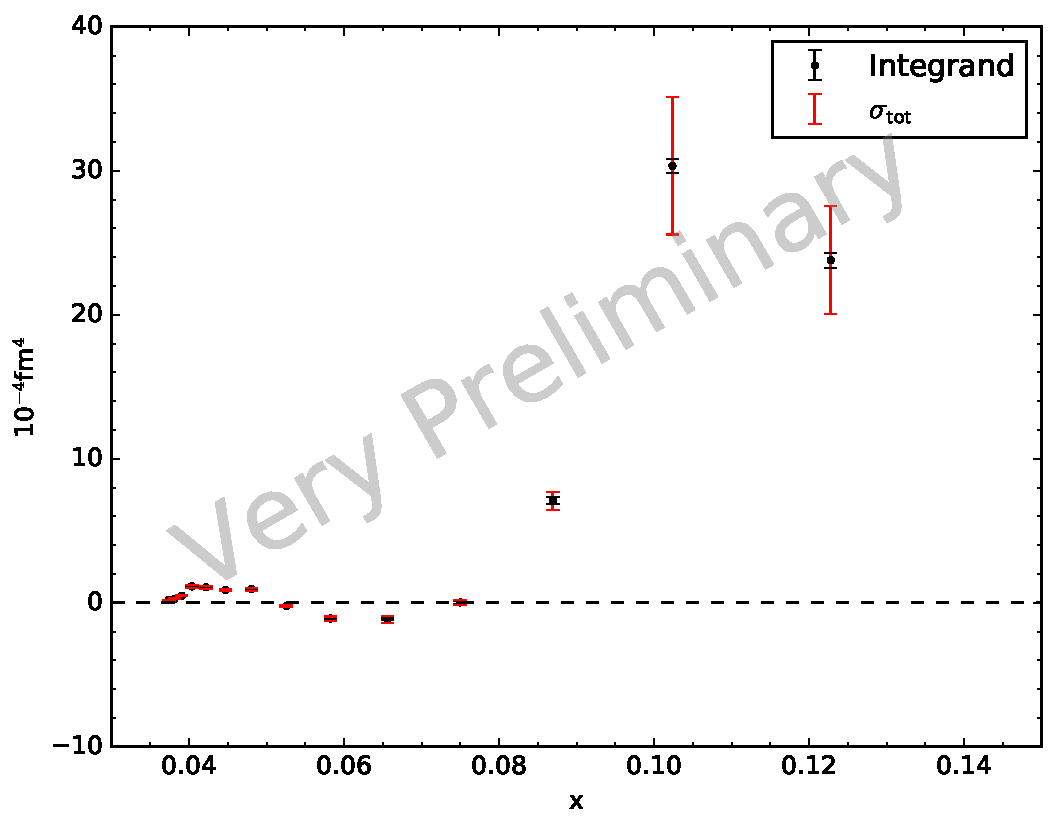
\includegraphics[width=\textwidth]{figs/gamma0-model-22535090.pdf}
    \caption{Transverse configuration. \label{C8S5F1b}}
  \end{subfigure}
  \caption[$\gamma_0$ integrand with $E=2.253$ GeV and $B=5.0$ T.]{Preliminary results for the $\gamma_0$ integrand for the kinematic setting with 2.253 GeV beam energy and 5.0 T target field (longitudinal and transverse configurations). For this setting, the average $Q^2$ is $\approx$0.1 GeV${}^2$. $\sigma_{\mathrm{tot}}$ is the total uncertainty. \label{C8S5F1}}
\end{figure}

\begin{figure}[p!]
  \centering
  \begin{subfigure}[t]{0.79\textwidth}
    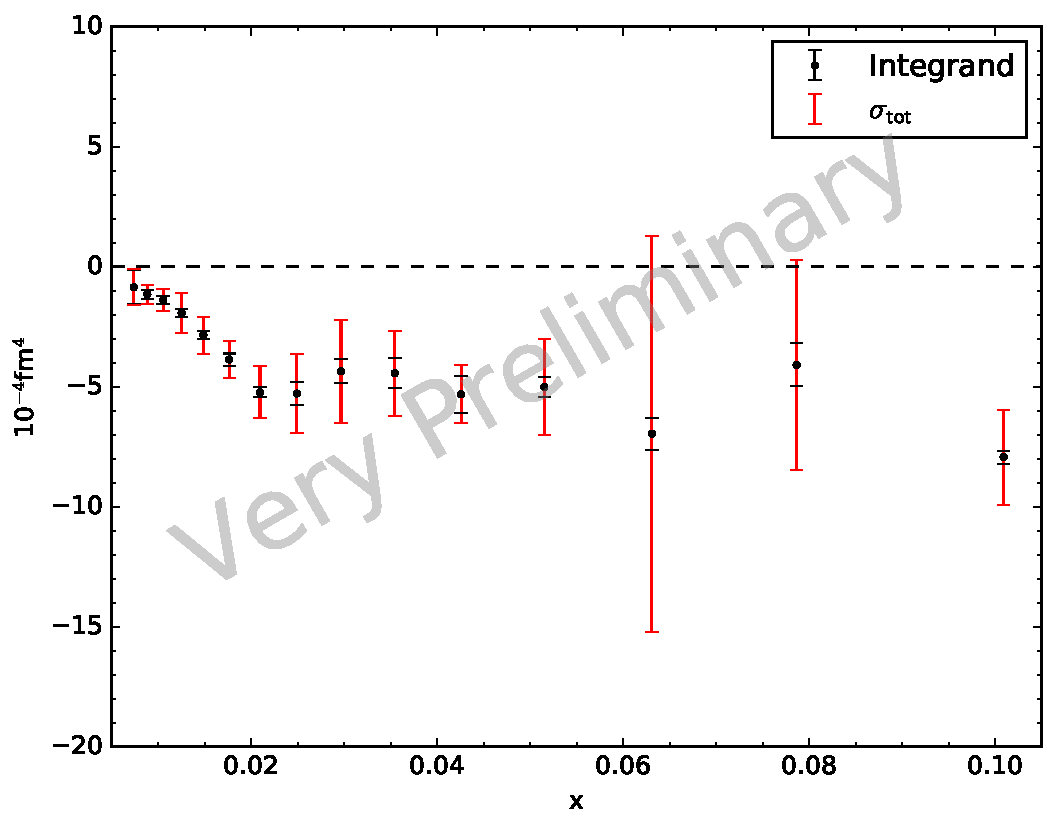
\includegraphics[width=\textwidth]{figs/dlt-model-22535000.pdf}
    \caption{Longitudinal configuration. \label{C8S5F2a}}
  \end{subfigure}
  \begin{subfigure}[t]{0.79\textwidth}
    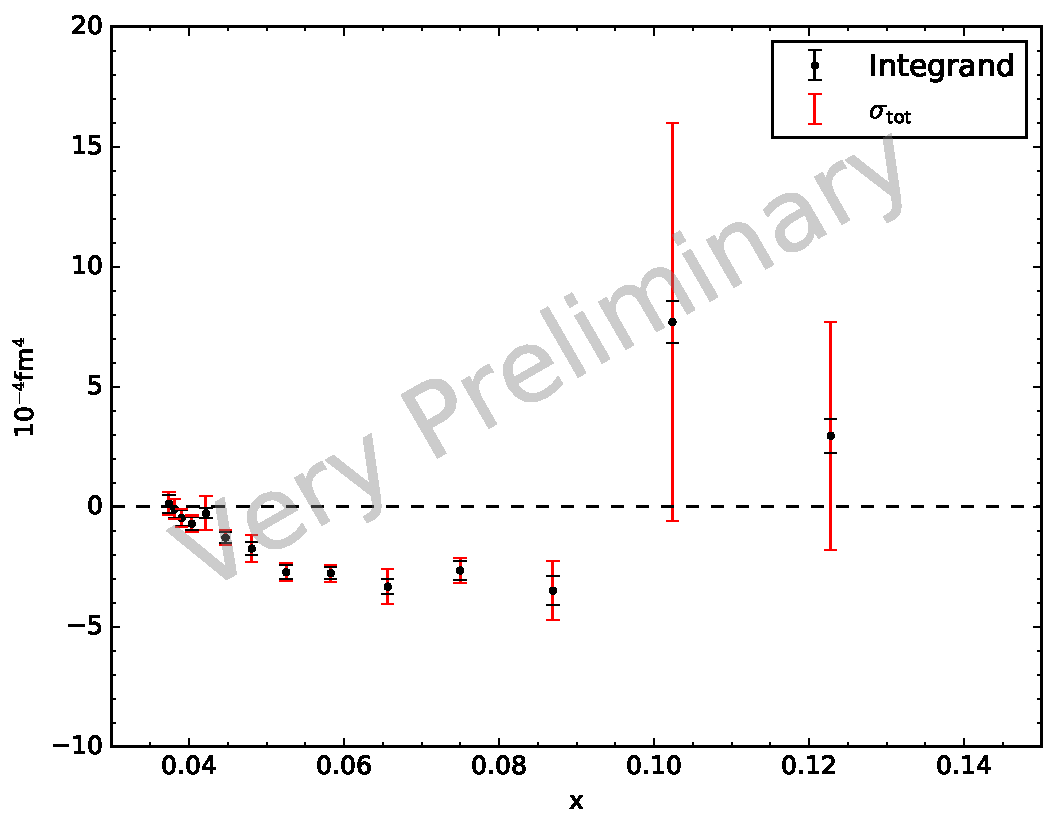
\includegraphics[width=\textwidth]{figs/dlt-model-22535090.pdf}
    \caption{Transverse configuration. \label{C8S5F2b}}
  \end{subfigure}
  \caption[$\dlt$ integrand with $E=2.253$ GeV and $B=5.0$ T.]{Preliminary results for the $\dlt$ integrand for the kinematic setting with 2.253 GeV beam energy and 5.0 T target field (longitudinal and transverse configurations). For this setting, the average $Q^2$ is $\approx$0.1 GeV${}^2$. $\sigma_{\mathrm{tot}}$ is the total uncertainty. \label{C8S5F2}}
\end{figure}

% \begin{figure}[p!]
%   \centering
%   \begin{subfigure}[t]{0.75\textwidth}
%     \includegraphics[width=\textwidth]{figs/gamma0-all.png}
%     \caption{Contribution to $\gamma_0$. \label{C8S5F3a}}
%   \end{subfigure}
%   \begin{subfigure}[t]{0.75\textwidth}
%     \includegraphics[width=\textwidth]{figs/dlt-all.png}
%     \caption{Contribution to $\dlt$. \label{C8S5F3b}}
%   \end{subfigure}
%   \caption[Contribution to the generalized spin polarizabilities from the resonance region.]{Contribution to the generalized spin polarizabilities from the resonance region. The unit is $10^{−4}$ fm${}^4$. \label{C8S5F3}}
% \end{figure}

As mentioned in \Cref{C2S4SS3}, the generalized polarizabilities $\gamma_0$ and $\dlt$ are moments of $g_1$ and $g_2$, \cref{C2S4SS3E8,C2S4SS3E12}. Using preliminary results for the spin structure functions presented in the previous section, we can calculate the integrand of $\gamma_0$ and $\dlt$. These results are shown in \cref{C8S5F1,C8S5F2}, for $\gamma_0$ and $\dlt$, respectively. Here only the two kinematic settings (longitudinal and transverse configurations) with 2.253 GeV beam energy and 5.0 T target field are shown as examples. The average $Q^2$ for this setting is $\approx$0.1 GeV${}^2$. To evaluate $\dlt$ and $\gamma_0$ at this $Q^2$, the integrals in \cref{C2S4SS3E8,C2S4SS3E12} have to be carried out from $x=0$ to the pion threshold, which is $x\approx0.25$ for this setting. The unmeasured low $x$ region will be evaluated using the $\gtww$ calculated from $g_1$ models. However, we expect the contribution of this low $x$ region to be suppressed due to the $x^2$ weighting in the integrals.

%The contribution to the $\gamma_0$ and $\dlt$ integral from the resonance region is shown in \Cref{C8S5F3} with the statistical and systematic uncertainties given with the data points.

\section{Conclusions and Future Work}
\label{C8S6}

The E08-027 collaboration successfully collected data for the first precision extraction of proton $g_2$ structure function in the $Q^2$ range of $0.02\sim0.2$ GeV${}^2$. The preliminary data analysis presented in this thesis has demonstrated that $g_2^p$ can be successfully extracted from E08-027 data, with the required precision for the calculation of $\gamma_0$, $\dlt$ for a stringent test of $\chi$PT predictions.

For preliminary results presented in this chapter, model predictions were used as inputs, for $\sigma_0$ in $\Delta\sigma_\perp$ and for $\Delta\sigma_\parallel$, to extract $g_2$ because the acceptance study of E08-027 has not been finalized. Once the acceptance study is finished, our data will be used to extract the unpolarized cross-sections $\sigma_0$ for each kinematic setting in place of the fits used here. In addition, the method for radiative correction in \Cref{C8S3} relies on the radiated cross-section models and thus is not sufficiently accurate. This method will be updated with the standard deconvolution method.

From preliminary results on the polarized cross-section differences $\Delta\sigma_\perp$, we can conclude that the data agree well with model predictions obtained from the MAID model and P. Bosted's fits in the region of the $\Delta$-resonance. However, the agreement for higher $W$ is not as good. From \Cref{C8S2F3}, we notice that the radiative effects are a large correction at high $W$, especially for the longitudinal configuration. This indicates that once we use our own data to extract the unpolarized cross-section and to perform the radiative correction, the agreement between calculation and data on $\Delta\sigma_{\perp,\parallel}$ may improve.

In \Cref{C8S4}, we used model predictions as inputs for $\Delta\sigma_{\parallel}$ since for most kinematics we measured only $\Delta\sigma_{\perp}$. The Jefferson Lab Hall B EG4 experiment measured $\Delta\sigma_{\parallel}$ in a similar kinematics range as this experiment. Thus, model predictions of $\Delta\sigma_{\parallel}$ will be replaced by data from EG4 once they finalize their analysis.

Once the studies mentioned above are done, the final results of the proton spin structure function $g_2$ will be extracted. These data will provide the first test of the BC sum rule for the proton at low $Q^2$. These data are also eagerly awaited to provide a benchmark test of the $\chi$PT predictions for the generalized spin polarizabilities $\gamma_0$ and $\dlt$.

%%%%%%%%%%%%%%%%%%%%%%%%%%%%%%%%%%%%%%%%%%%%%%%%%%%%%%%%%%%%%%%%%%%%%%
% -*-latex-*-
